\chapter{Appendix}

\section{Overview}

This chapter describes how several of the identified vulnerabilities can be combined to compromise the target system. 
\\

It presents the main attack paths observed during the assessment, from the initial access vector through exploitation and privilege escalation, and summarizes the resulting impact on the target environment. 

\section{Exploiting several vulnerabilities}

The penetration testing activity resulted in the successful compromise of the target system through a multi-stage attack chain involving vulnerabilities in the exposed web application, insecure handling of system log files, insufficient protection of sensitive backup data, and a local privilege escalation vulnerability.

\subsection{Identifying Potential Entry Points}
The initial attack surface was identified through enumeration of the web application. Several accessible directories and files were discovered, including \texttt{/blog-post/archives/}, \texttt{/blog-post/uploads/}, \texttt{/tasks/}, \texttt{randylogs.php}, and \texttt{tasks\_todo.txt}.
\\

While some of these resources did not directly provide access to the underlying system, they disclosed information that enabled further vulnerability analysis. In particular, \texttt{tasks\_todo.txt} contained information referring to the \texttt{/var/log/auth.log} file. 
\\

This information, combined with the discovery of \texttt{randylogs.php}, provided a strong indication that the application contained functionality for retrieving system log files.

\subsection{Initial Access Through Local File Inclusion}

Direct requests to \texttt{randylogs.php} returned an empty response, suggesting that the application required an input parameter. Parameter fuzzing with \texttt{wfuzz} identified the \texttt{file} parameter as the relevant input accepted by the PHP script.

\begin{figure}[H]
\centering
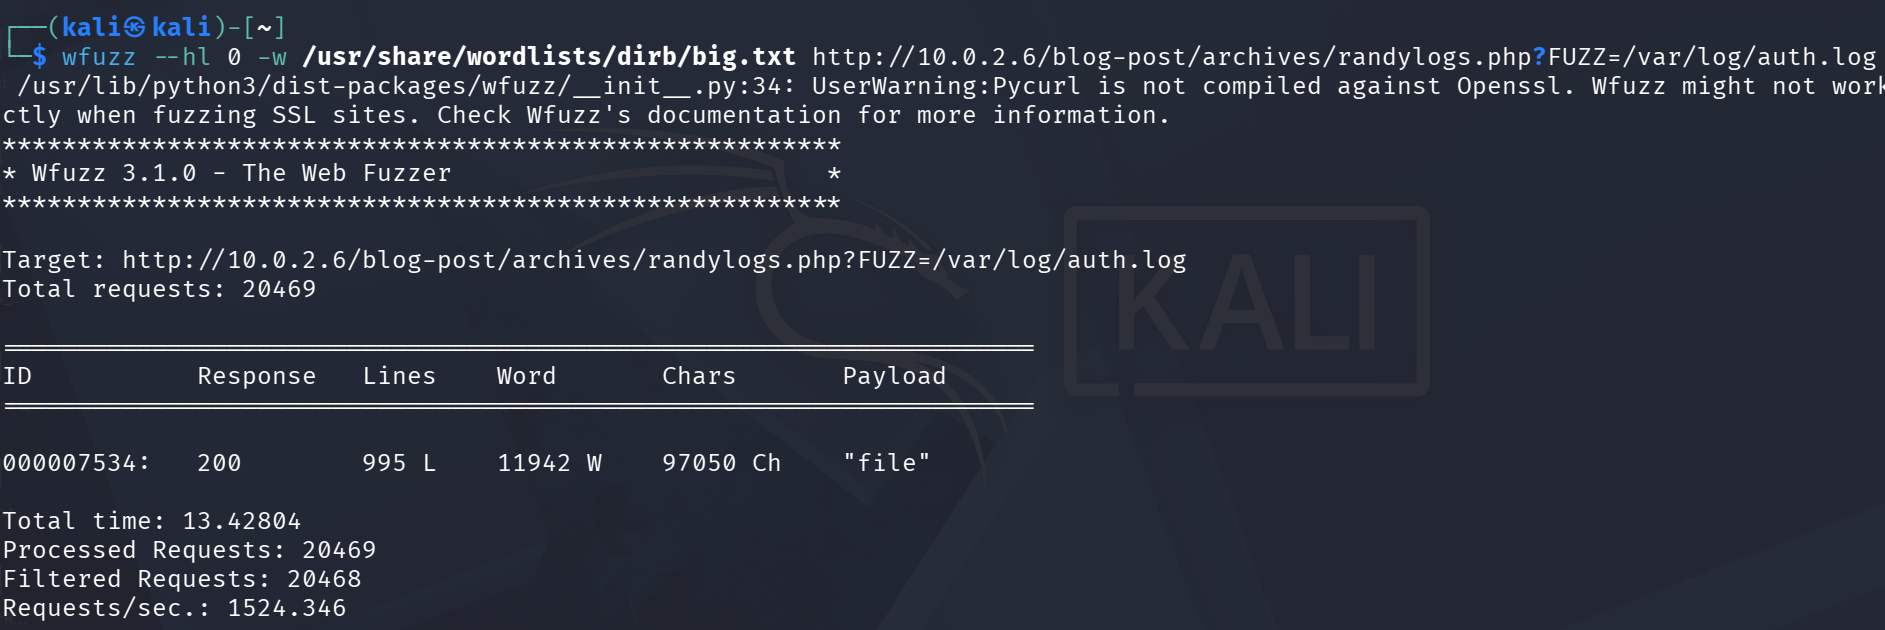
\includegraphics[width=0.75\linewidth]{GlobalAssets/randylogsphpfuzz.png}
\caption{Identification of the \texttt{file} parameter through parameter fuzzing}
\label{fig:detailed-lfi-fuzzing}
\end{figure}

The parameter was subsequently tested using the path to the authentication log referenced by \texttt{tasks\_todo.txt}. The following request successfully retrieved the contents of the local file:

\begin{verbatim}
http://10.0.2.6/blog-post/archives/randylogs.php?file=/var/log/auth.log
\end{verbatim}

\begin{figure}[H]
\centering
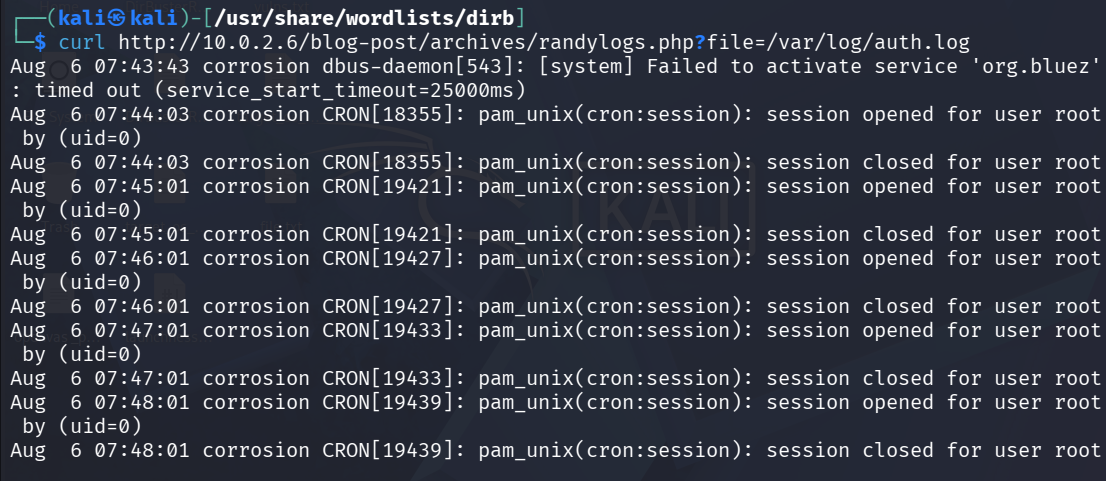
\includegraphics[width=0.75\linewidth]{GlobalAssets/authlogcontent.png}
\caption{Successful retrieval of \texttt{/var/log/auth.log} through the web application}
\label{fig:detailed-authlog}
\end{figure}

This behavior confirms a \textbf{Local File Inclusion (LFI)} vulnerability. The application passes a user-controlled filesystem path to functionality that reads or includes the specified file without enforcing an appropriate restriction on the accessible path.
\\

The impact of this vulnerability is significant because the affected functionality is not restricted to application resources. An attacker can request arbitrary files readable by the web server process, potentially exposing configuration files, credentials, logs, source code, and other sensitive information stored on the underlying operating system.

\subsection{LFI-to-RCE Escalation Through Log Poisoning}

The contents of \texttt{/var/log/auth.log} showed that the file records SSH authentication activity. This introduced the possibility of using the log file as a controllable input source.
\\

The attack consisted of two stages. First, attacker-controlled data had to be written into \texttt{/var/log/auth.log}. Second, the poisoned log had to be processed as PHP code through the existing LFI vulnerability.
\\

An initial attempt was made to inject PHP code through the SSH username field. This approach was unsuccessful because the SSH implementation rejected the characters required to construct the PHP payload.

\begin{figure}[H]
\centering
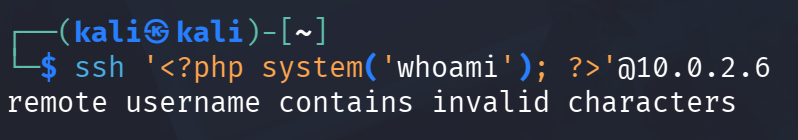
\includegraphics[width=0.75\linewidth]{GlobalAssets/sshinvalidchar.png}
\caption{Unsuccessful attempt to inject PHP code through the SSH username field}
\label{fig:detailed-ssh-injection}
\end{figure}

An alternative method was therefore used to introduce attacker-controlled content into the target environment through the available SFTP functionality. This allowed the required payload to be written to a location subsequently processed through the LFI vulnerability.

\begin{figure}[H]
\centering
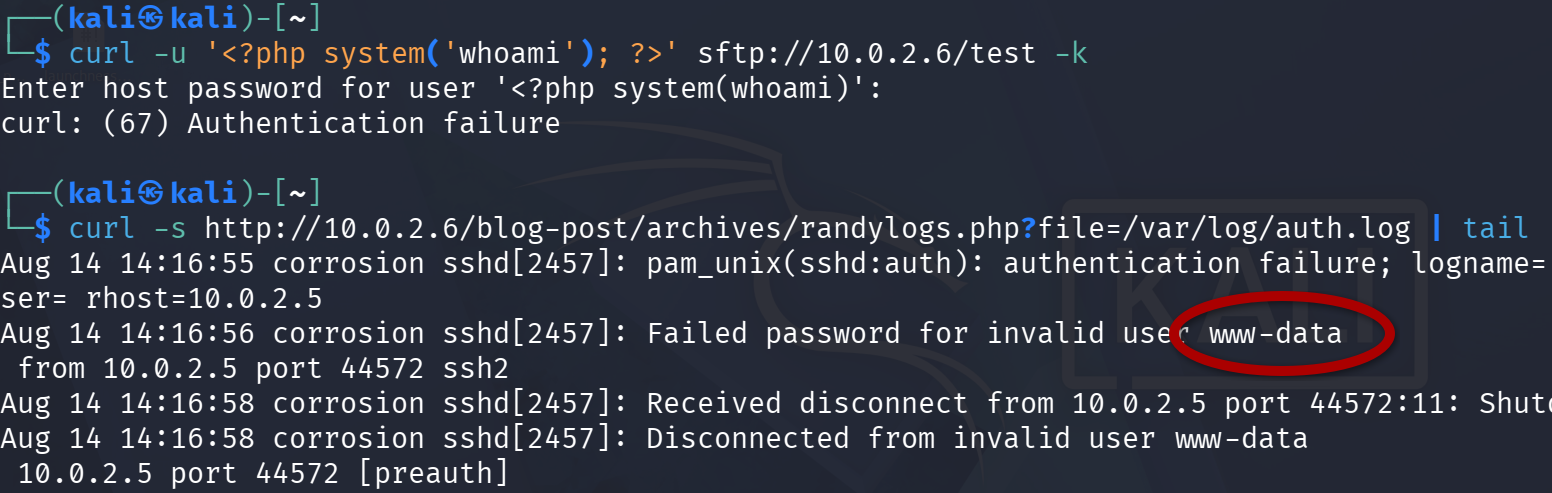
\includegraphics[width=0.75\linewidth]{GlobalAssets/rcesuccess.png}
\caption{Successful exploitation of the LFI vulnerability to achieve code execution}
\label{fig:detailed-lfi-rce}
\end{figure}

The resulting behavior demonstrated that the LFI was not limited to arbitrary file disclosure. Because the included file could contain attacker-controlled PHP code, the vulnerability could be escalated to \textbf{Remote Code Execution (RCE)}.
\\

For exploitation, the injected PHP functionality was designed to accept a second HTTP parameter, \texttt{cmd}, and execute its value using the PHP \texttt{system()} function. This transformed the original arbitrary-file-inclusion primitive into a command-execution primitive.
\\

The resulting attack chain can therefore be summarized as:

\begin{enumerate}
    \item Attacker-controlled input through SFTP;
    \item Poisoned \texttt{/var/log/auth.log} file;
    \item \texttt{randylogs.php?file=<controlled file>};
    \item PHP interpretation of injected content;
    \item Remote command execution.
\end{enumerate}

\subsection{Establishing a Reverse Shell}
To obtain an interactive foothold on the target, a Bash reverse-shell payload was supplied through the \texttt{cmd} parameter. The target was instructed to initiate a TCP connection to the attacking machine at \texttt{10.0.2.5:9000}.
\\

The attacking machine was first configured to listen for the incoming connection using \texttt{netcat}:

\begin{verbatim}
nc -nlvp 9000
\end{verbatim}

\begin{figure}[H]
\centering
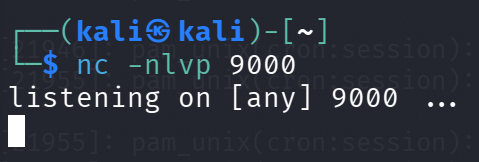
\includegraphics[width=0.50\linewidth]{GlobalAssets/netcat1.png}
\caption{Netcat listener waiting for the reverse-shell connection}
\label{fig:detailed-netcat}
\end{figure}

The malicious command was then supplied to the vulnerable PHP script. When the poisoned file was processed, the injected PHP code executed the command and caused the target to establish the outbound connection.

\begin{figure}[H]
\centering
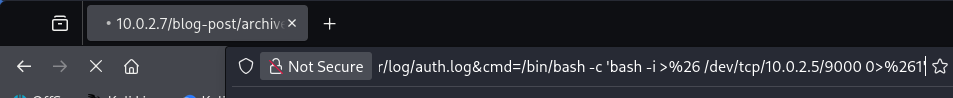
\includegraphics[width=0.75\linewidth]{GlobalAssets/attackfirefox.png}
\caption{Delivery of the command-execution request}
\label{fig:detailed-request}
\end{figure}

The resulting connection provided an interactive shell on the target system.

\begin{figure}[H]
\centering
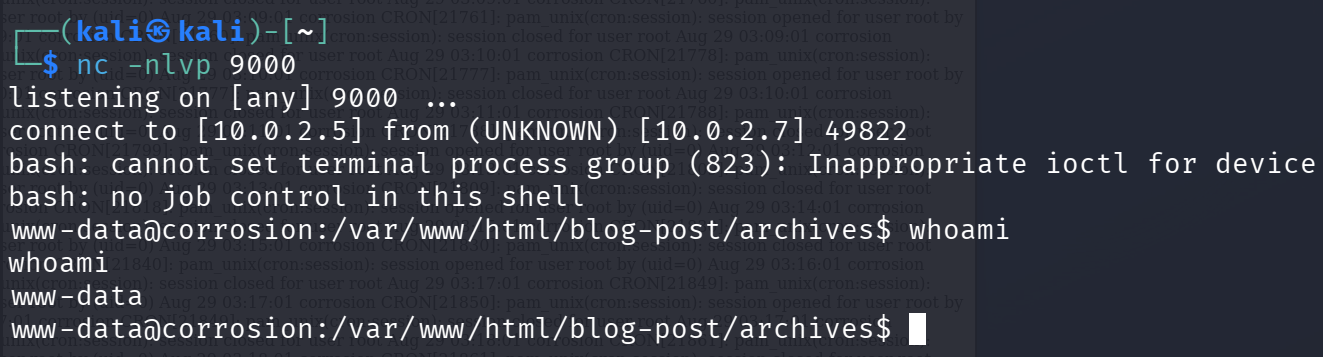
\includegraphics[width=0.75\linewidth]{GlobalAssets/reverseshellsuccess.png}
\caption{Successful establishment of the reverse shell}
\label{fig:detailed-reverse-shell}
\end{figure}

At this stage, remote code execution had been successfully converted into an interactive foothold on the target. The shell initially operated with the privileges of the web application process, providing a low-privileged context from which local privilege escalation and further enumeration could be performed.

\subsection{Post-Exploitation and Credential Discovery}

Following establishment of the reverse shell, local enumeration was performed to identify users, sensitive files, and potential privilege escalation vectors.
\\

Inspection of \texttt{/etc/passwd} revealed the presence of the \texttt{randy} user account.

\begin{figure}[H]
\centering
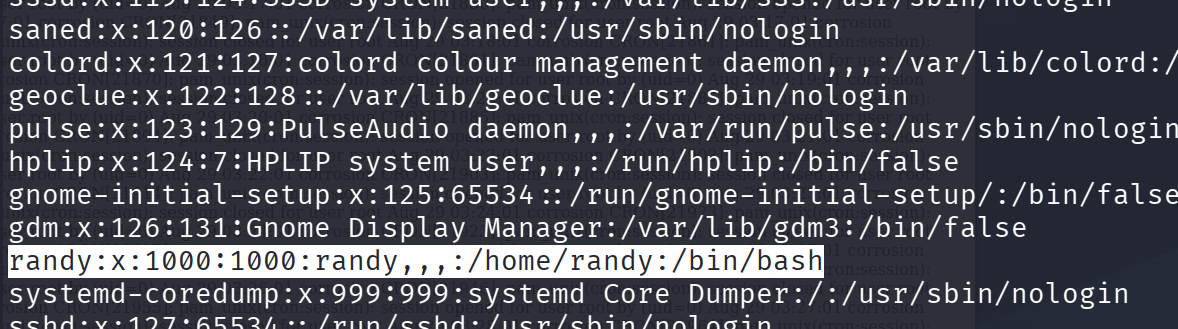
\includegraphics[width=0.75\linewidth]{GlobalAssets/userrandy.png}
\caption{Identification of the \texttt{randy} user account}
\label{fig:detailed-randy}
\end{figure}

Further filesystem enumeration identified \texttt{user\_backup.zip} within \texttt{/var/backups/}. The archive was password-protected and could not initially be extracted.

\begin{figure}[H]
\centering
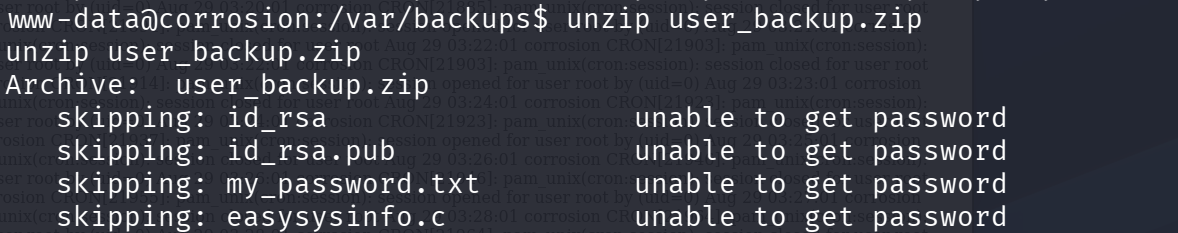
\includegraphics[width=0.75\linewidth]{GlobalAssets/unzipfail.png}
\caption{Password protection preventing extraction of \texttt{user\_backup.zip}}
\label{fig:detailed-zip-protected}
\end{figure}

Because the archive was accessible from the compromised system and potentially contained authentication material, it was selected for further analysis.
\\

The archive was transferred to the attacking machine and subjected to password recovery using \texttt{zip2john} and \texttt{John the Ripper}. The password was successfully recovered.

\begin{figure}[H]
\centering
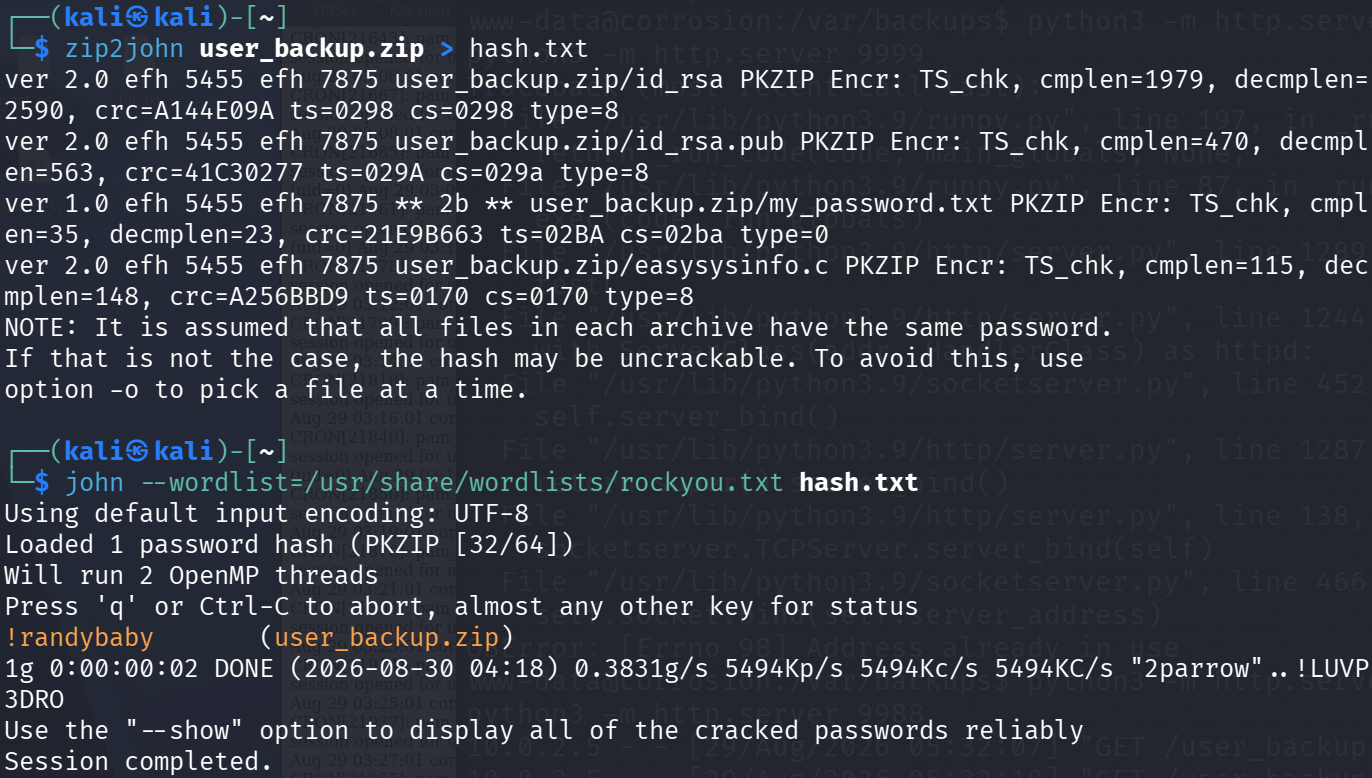
\includegraphics[width=0.75\linewidth]{GlobalAssets/randybaby.png}
\caption{Recovery of the password protecting the backup archive}
\label{fig:detailed-password-cracking}
\end{figure}

Extraction of the archive revealed several sensitive files:

\begin{itemize}
\item \texttt{id\_rsa}, containing a private SSH key;
\item \texttt{id\_rsa.pub}, containing the corresponding public key;
\item \texttt{my\_password.txt}, containing a user password;
\item \texttt{easysysinfo.c}, containing the source code of a privileged utility.
\end{itemize}

\begin{figure}[H]
\centering
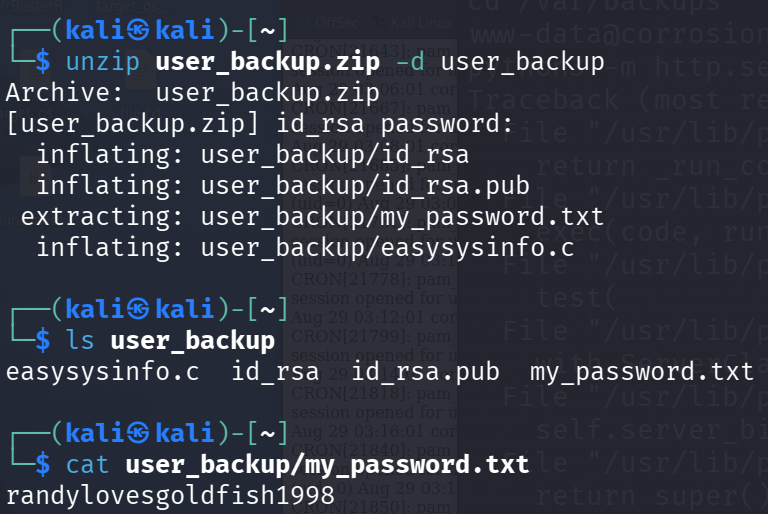
\includegraphics[width=0.50\linewidth]{GlobalAssets/zipcracked.png}
\caption{Sensitive contents recovered from \texttt{user\_backup.zip}}
\label{fig:detailed-zip-content}
\end{figure}

The password contained in \texttt{my\_password.txt} enabled authentication to the \texttt{randy} account.

\begin{figure}[H]
\centering
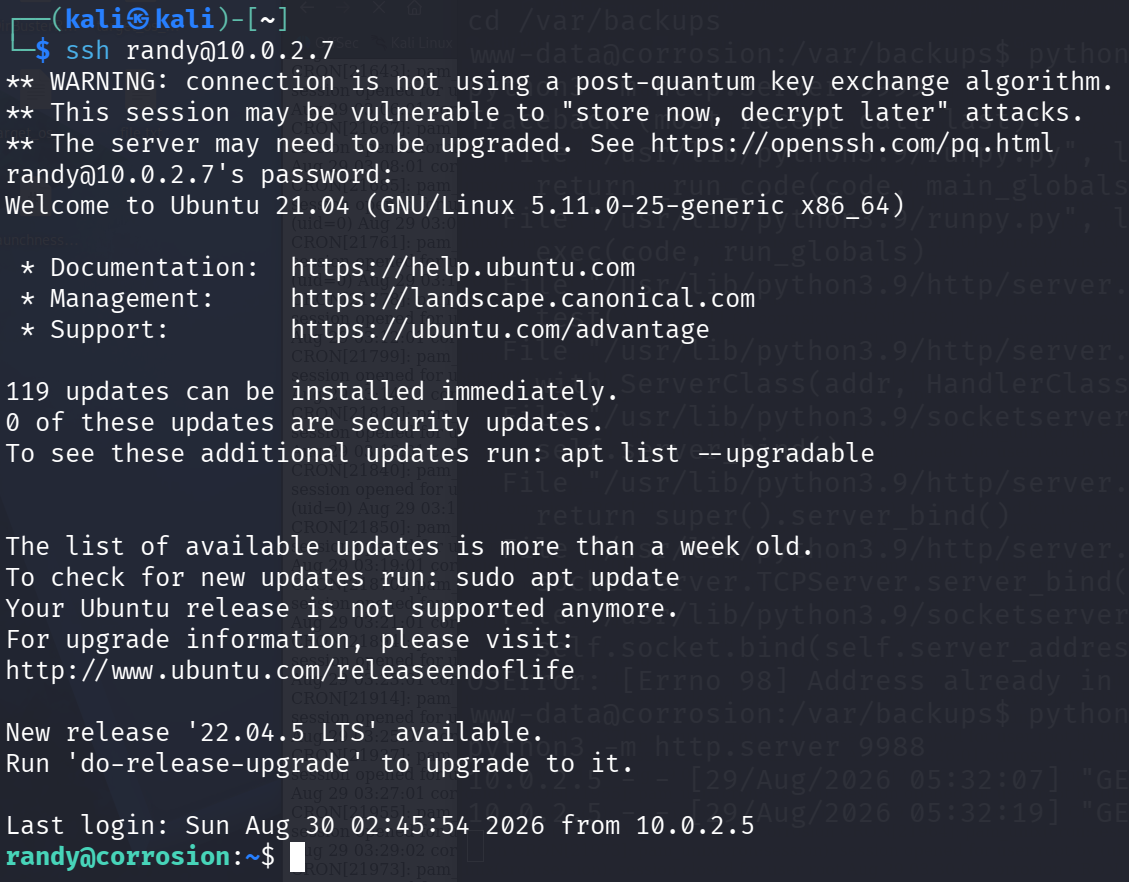
\includegraphics[width=0.75\linewidth]{GlobalAssets/randylogin.png}
\caption{Successful authentication as the \texttt{randy} user}
\label{fig:detailed-randy-login}
\end{figure}

This represented a privilege transition from the web application's low-privileged execution context to a legitimate local user account.

\subsection{Local Privilege Escalation}

Enumeration of the \texttt{randy} user's environment identified the \texttt{easysysinfo} utility within the user's \texttt{tools} directory.

\begin{figure}[H]
\centering
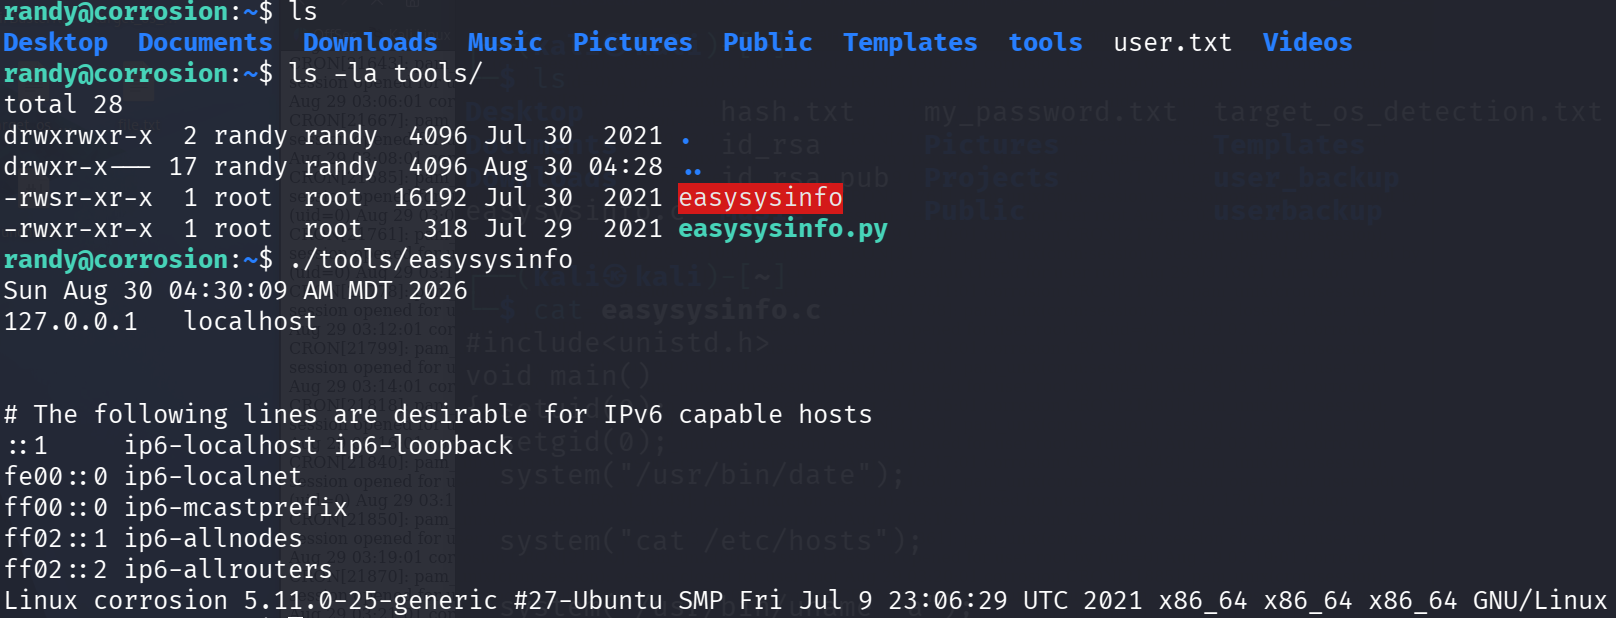
\includegraphics[width=0.75\linewidth]{GlobalAssets/exploring.png}
\caption{Enumeration of the \texttt{randy} user's environment}
\label{fig:detailed-randy-enumeration}
\end{figure}

The executable had \texttt{setuid} permissions, meaning that it executed with the effective privileges of its file owner rather than solely with the privileges of the invoking user. 
\\

Further analysis showed that the program was owned by \texttt{root} and therefore represented a potential privilege escalation vector.
\\

The corresponding source code found in the \texttt{user\_backup.zip} archive revealed the use of the C \texttt{system()} function to invoke the \texttt{cat} utility.

\begin{figure}[H]
\centering
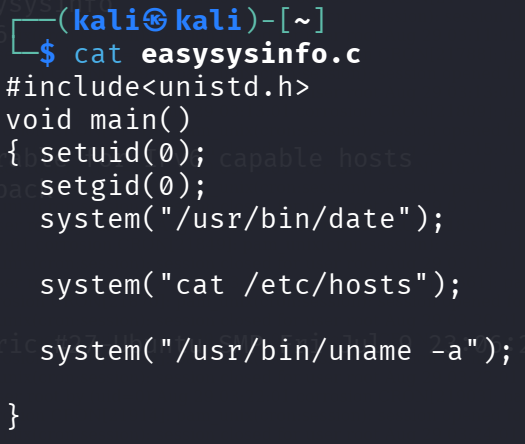
\includegraphics[width=0.40\linewidth]{GlobalAssets/easysysinfo.png}
\caption{Source code of the \texttt{easysysinfo} utility}
\label{fig:detailed-easysysinfo}
\end{figure}

The security weakness results from the use of an external executable without specifying its absolute filesystem path. Instead of explicitly invoking a trusted executable such as \texttt{/bin/cat}, the program relies on the \texttt{PATH} environment variable to determine which executable should be executed.
\\

This behavior is classified as \textbf{CWE-426: Untrusted Search Path}. An attacker able to influence the execution environment can cause a malicious executable to be resolved in place of the intended system binary.
\\

Because the vulnerable program executes with root privileges, successful manipulation of executable resolution causes the attacker-controlled program to inherit those privileges.

\subsection{Root Privilege Escalation}

To demonstrate the impact of the vulnerable search-path behavior, a malicious executable named \texttt{cat} was created.

\begin{figure}[H]
\centering
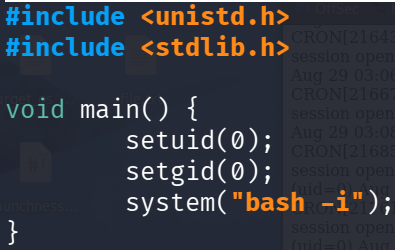
\includegraphics[width=0.40\linewidth]{GlobalAssets/fakecat.png}
\caption{Creation of the malicious \texttt{cat} executable}
\label{fig:detailed-fakecat}
\end{figure}

The executable was placed in \texttt{/tmp}, and the \texttt{PATH} environment variable was modified so that \texttt{/tmp} was searched before the directory containing the legitimate \texttt{cat} executable.
\\

Consequently, when \texttt{easysysinfo} invoked \texttt{cat}, the malicious executable was resolved instead of the legitimate system binary.
\\

Since \texttt{easysysinfo} executes with root privileges, the attacker-controlled process inherited the corresponding effective privileges. Execution of the utility therefore resulted in a \textbf{root shell}.

\begin{figure}[H]
\centering
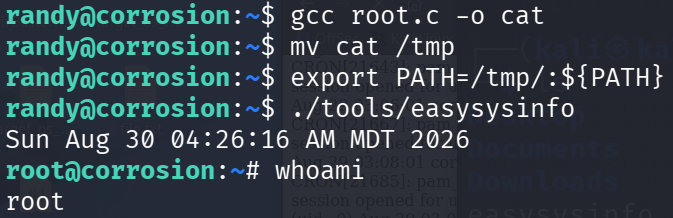
\includegraphics[width=0.75\linewidth]{GlobalAssets/rooted.png}
\caption{Successful local privilege escalation to root}
\label{fig:detailed-root}
\end{figure}

The successful privilege escalation demonstrates that the initial web application compromise could ultimately be converted into complete operating-system-level takeover.

